\documentclass[11pt,a4paper]{article}

\usepackage[spanish,es-nodecimaldot,es-tabla]{babel}
\usepackage{fontspec}
\usepackage{amsmath}
\usepackage{siunitx}
\usepackage{booktabs}
\usepackage{graphicx}
\usepackage{float}
\usepackage[font=small,labelfont=bf]{caption}
\usepackage[margin=2.4cm]{geometry}
\usepackage{microtype}
\usepackage[hidelinks]{hyperref}

\sisetup{output-decimal-marker={.}, group-separator={\,}, group-minimum-digits=4}
\graphicspath{{fotos/}{../resultados/}}

\newcommand{\autor}{Sebastian Velandia Acevedo y Jesus Martinez}

\title{Astronomía para Todos\\[4pt]\large Taller de ejercicios sobre magnitudes}
\author{\autor}
\date{3 de noviembre de 2026}

\begin{document}
\maketitle
\tableofcontents

% =====================================================================
\section{Punto 1: un tren a \texorpdfstring{$\alpha$}{alfa}~Centauri}

\begin{figure}[H]
\centering
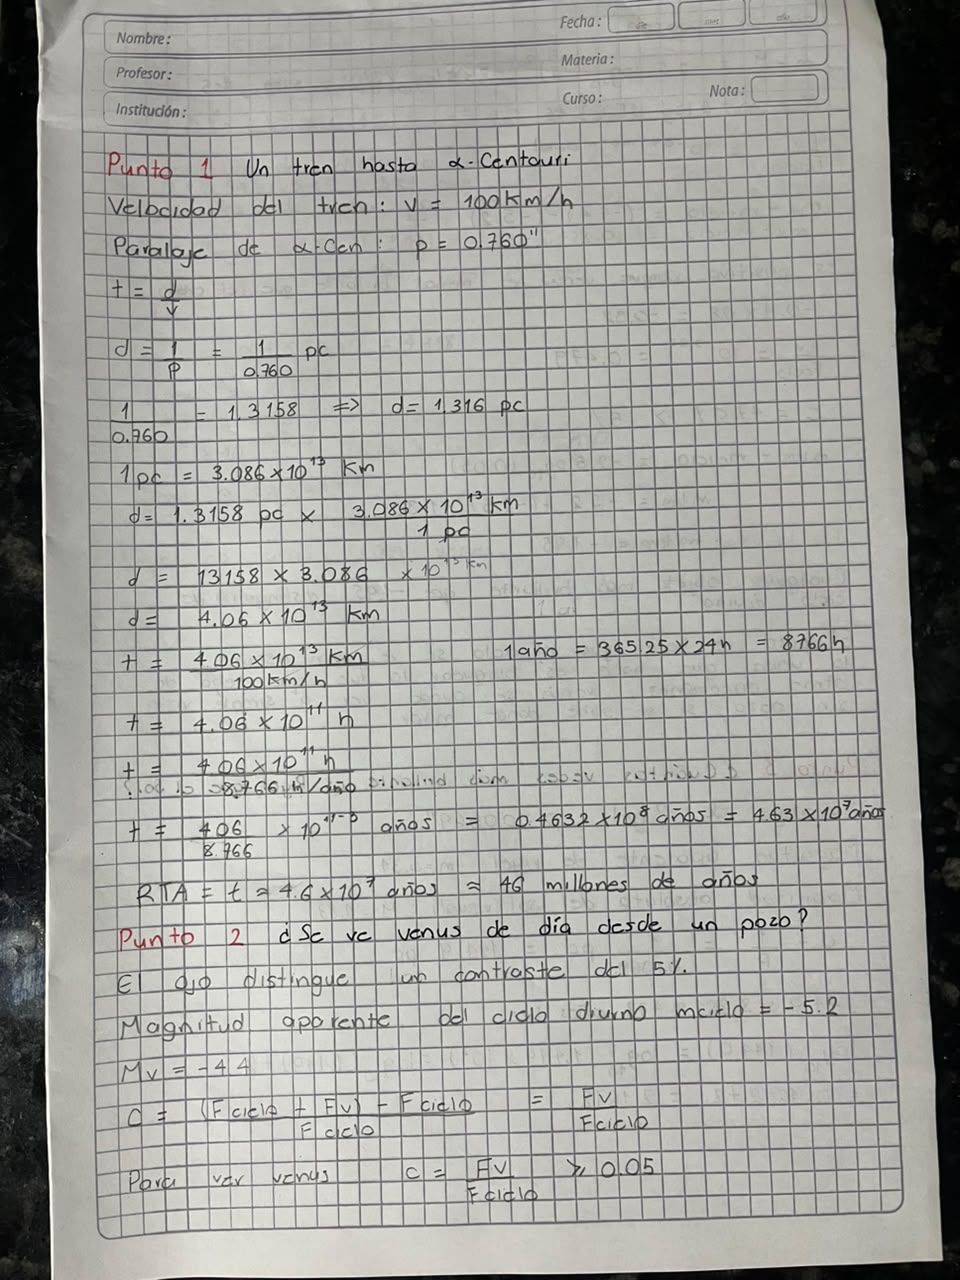
\includegraphics[height=0.80\textheight]{hoja1_puntos1_2.jpg}
\caption{Desarrollo del punto 1 y comienzo del punto 2.}
\end{figure}

\textbf{Respuesta:} el tren tardaría unos $\num{4.6e7}$ años, es decir, unos \textbf{46 millones de años}.

% =====================================================================
\section{Punto 2: ¿Venus de día desde el fondo de un pozo?}

\begin{figure}[H]
\centering
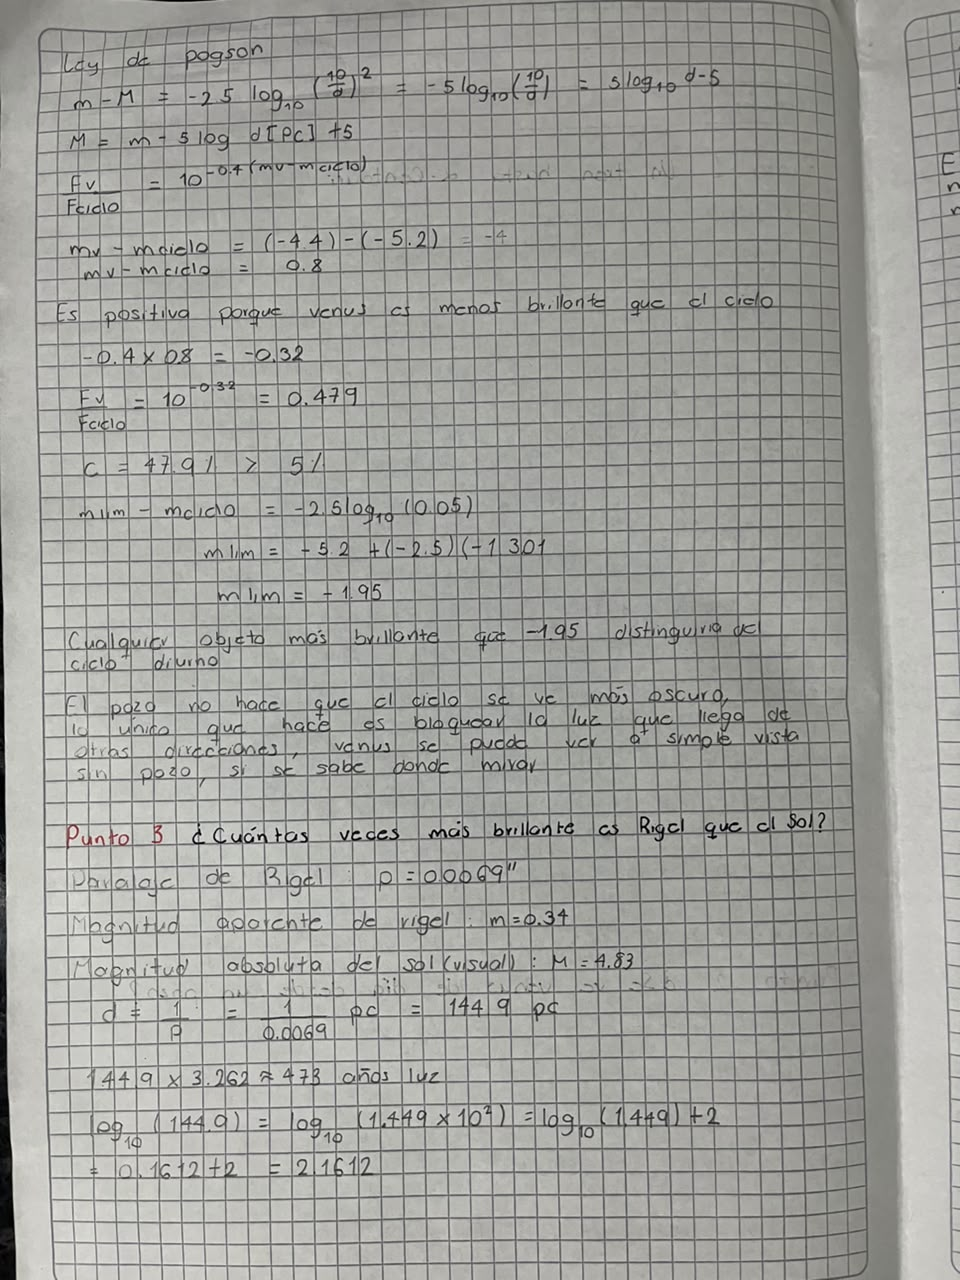
\includegraphics[height=0.80\textheight]{hoja2_puntos2_3.jpg}
\caption{Continuación del punto 2 y comienzo del punto 3.}
\end{figure}

El valor $m_V = -4.4$ es la magnitud de Venus en su máximo brillo, que llega a $-4.4$ a $-4.6$
\cite{naoj,earthsky}.

Además del brillo, hay que ver qué parte del cielo se alcanza a ver desde el pozo. Desde el fondo de un pozo profundo solo se
ve una zona pequeña del cielo alrededor del cenit: un pozo de \SI{1}{m} de diámetro y \SI{20}{m} de
profundidad muestra un círculo de $\arctan(0.5/20) \approx 1.4^\circ$ de radio. Venus nunca se aleja más
de unos $27$--$28^\circ$ del ecuador celeste (la eclíptica está inclinada $23.4^\circ$ y la órbita de
Venus otros $3.4^\circ$). En Albania, a unos $41^\circ$ de latitud norte, Venus pasa como mínimo a unos
$41^\circ - 28^\circ = 13^\circ$ del cenit, así que nunca entra en el trozo de cielo visible desde el
fondo del pozo.

\textbf{Respuesta: no es cierto.} Por su brillo, Venus sí se puede ver de día (su
contraste con el cielo, 47.9\,\%, es casi diez veces el 5\,\% que distingue el ojo), y se ve sin
necesidad de un pozo. El pozo no hace que el cielo se vea más oscuro, y además desde el fondo de un pozo profundo en
Albania Venus nunca pasaría por la zona de cielo visible.

% =====================================================================
\section{Punto 3: ¿cuántas veces más brillante es Rigel que el Sol?}

\begin{figure}[H]
\centering
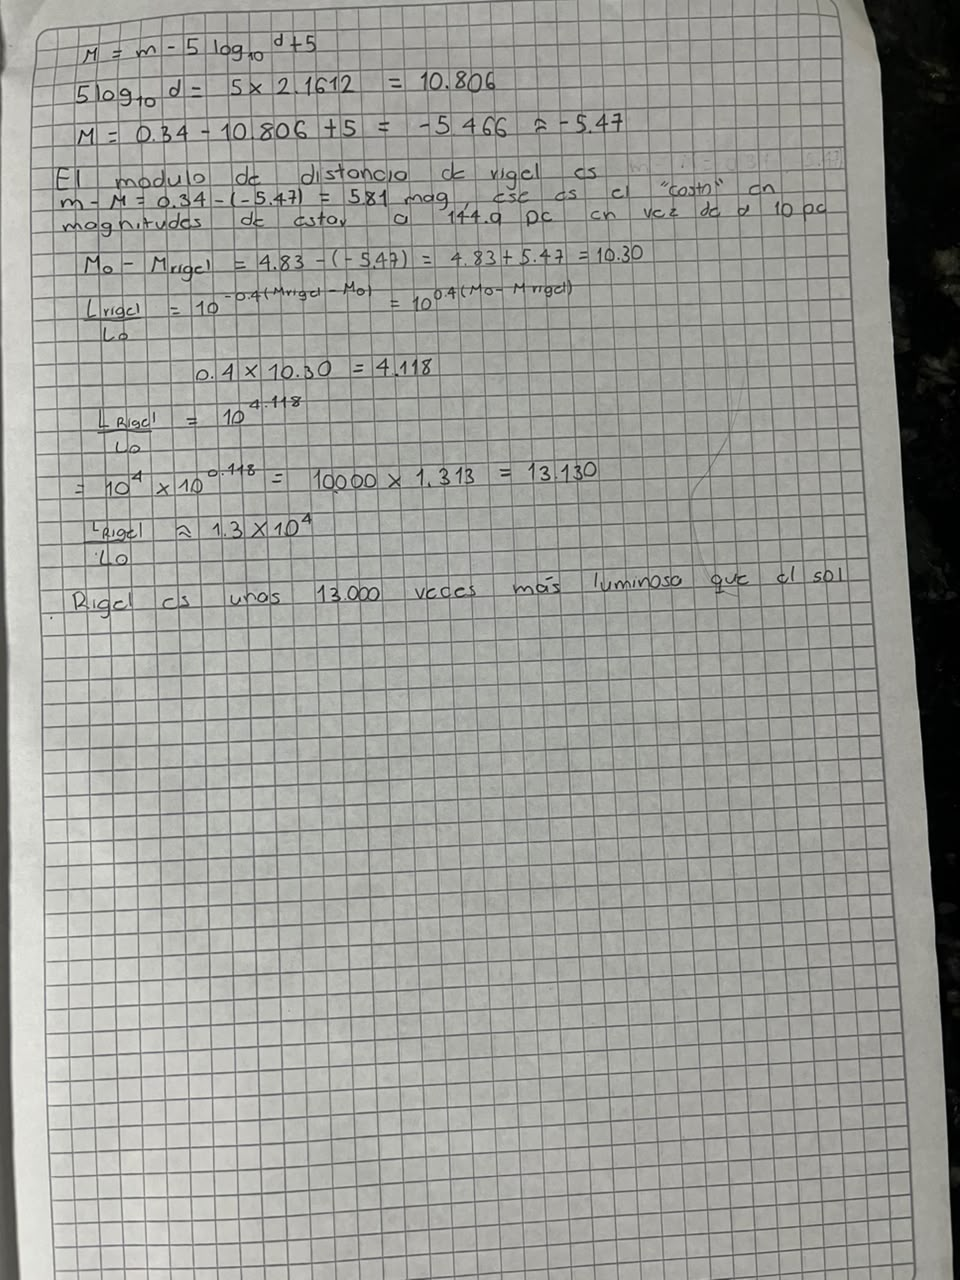
\includegraphics[height=0.80\textheight]{hoja3_punto3.jpg}
\caption{Final del punto 3.}
\end{figure}

\textbf{Respuesta:} Rigel es unas \textbf{\num{13000} veces más luminoso que el Sol} en luz visible. Como
usamos la magnitud del Sol en visible (4.83), esto compara solo la luz visible. Rigel es una supergigante azul (B8\,Ia) que emite mucho en el
ultravioleta, así que su luminosidad total es aún mayor.

% =====================================================================
\section{Punto 4: la Gran Nube de Magallanes}

La Gran Nube de Magallanes (LMC) está a \SI{50}{kpc}. Sus datos de referencia se resumen en la
tabla~\ref{tab:ref}.

No usamos los servicios del CDS (Centro de Datos Astronómicos de Estrasburgo), de donde Aladin descarga
normalmente los surveys y los catálogos, porque estuvieron caídos durante todo el tiempo en que hicimos
el taller, desde el 28 de octubre de 2026. Nos tocó usar alternativas: las imágenes del servicio
SkyView de la NASA, la consulta a SIMBAD a través de su espejo de la Universidad de Harvard y, para el
catálogo de Bonanos et al., la tabla original publicada por la revista, que es la misma que distribuye
VizieR. En óptico usamos el mosaico de Mellinger en lugar del DSS que pide el enunciado. Para un campo
tan grande, SkyView arma el DSS juntando placas fotográficas con fondos distintos, que dejan escalones
de brillo y no permiten medir la galaxia.

\begin{table}[H]
\centering
\caption{Datos de referencia de la LMC y de la Nebulosa de la Tarántula.}
\label{tab:ref}
\begin{tabular}{lll}
\toprule
Propiedad & Valor & Fuente \\
\midrule
Coordenadas (J2000) & $05^\text{h}23^\text{m}34.6^\text{s}$, $-69^\circ45'22''$ & SIMBAD \cite{simbad} \\
Tamaño (óptico) & $322.8' \times 274.8' = 5.38^\circ \times 4.58^\circ$ & SIMBAD \cite{simbad} \\
Tamaño $D_{25}$ (filtro B) & $645.7' \times 549.5' = 10.76^\circ \times 9.16^\circ$ & RC3 \cite{rc3} \\
Nebulosa 30 Doradus & $40' \times 25'$ & SIMBAD \cite{simbad} \\
\bottomrule
\end{tabular}
\end{table}

El tamaño $D_{25}$ se mide hasta la isofota de 25~mag\,arcsec$^{-2}$ en el filtro B e incluye el disco
externo débil; el de SIMBAD corresponde a la parte brillante.

\subsection{Imágenes en óptico, infrarrojo, radio y rayos gamma}
Se visualizó la región en campos de $20^\circ \times 20^\circ$ en Aladin Desktop \cite{aladin}, con
imágenes del servicio SkyView de la NASA (figura~\ref{fig:bandas}):
\begin{itemize}
  \item óptico: mosaico de Mellinger \cite{mellinger};
  \item infrarrojo: AKARI a \SI{140}{\micro m} \cite{akari};
  \item submilimétrico y radio: Planck a \SI{857}{GHz} y a \SI{30}{GHz} \cite{planck};
  \item rayos gamma: Fermi-LAT \cite{fermi}.
\end{itemize}
El canal de \SI{857}{GHz} de Planck es submilimétrico y muestra emisión térmica de polvo; el de
\SI{30}{GHz} es el que corresponde a radio.

\begin{figure}[H]
\centering
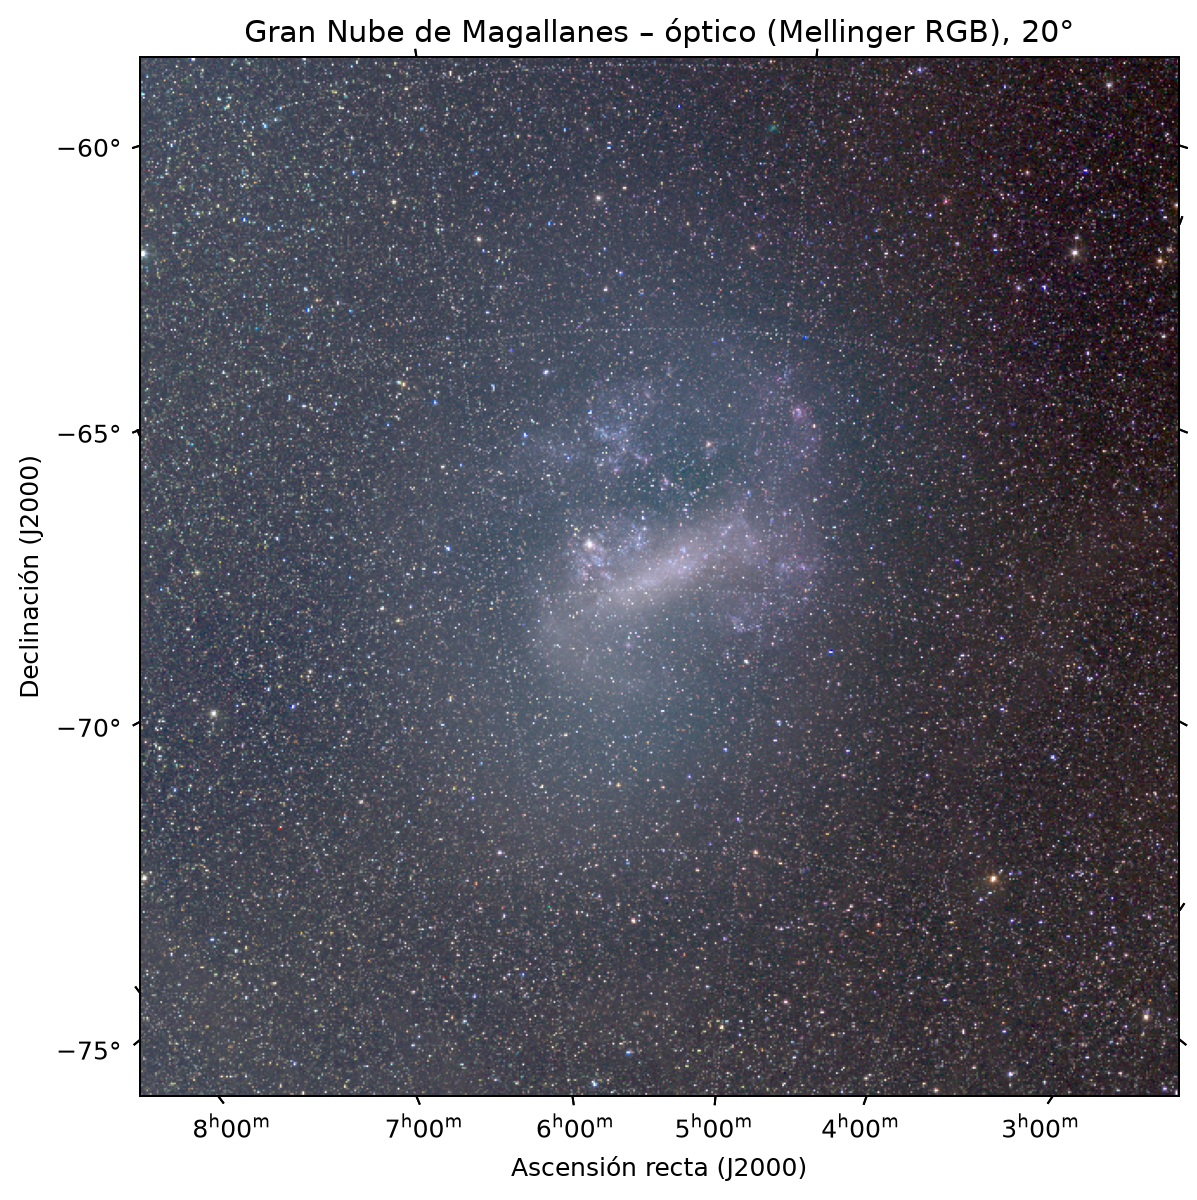
\includegraphics[width=0.40\textwidth]{punto4/LMC_optico_Mellinger_color_20deg.png}
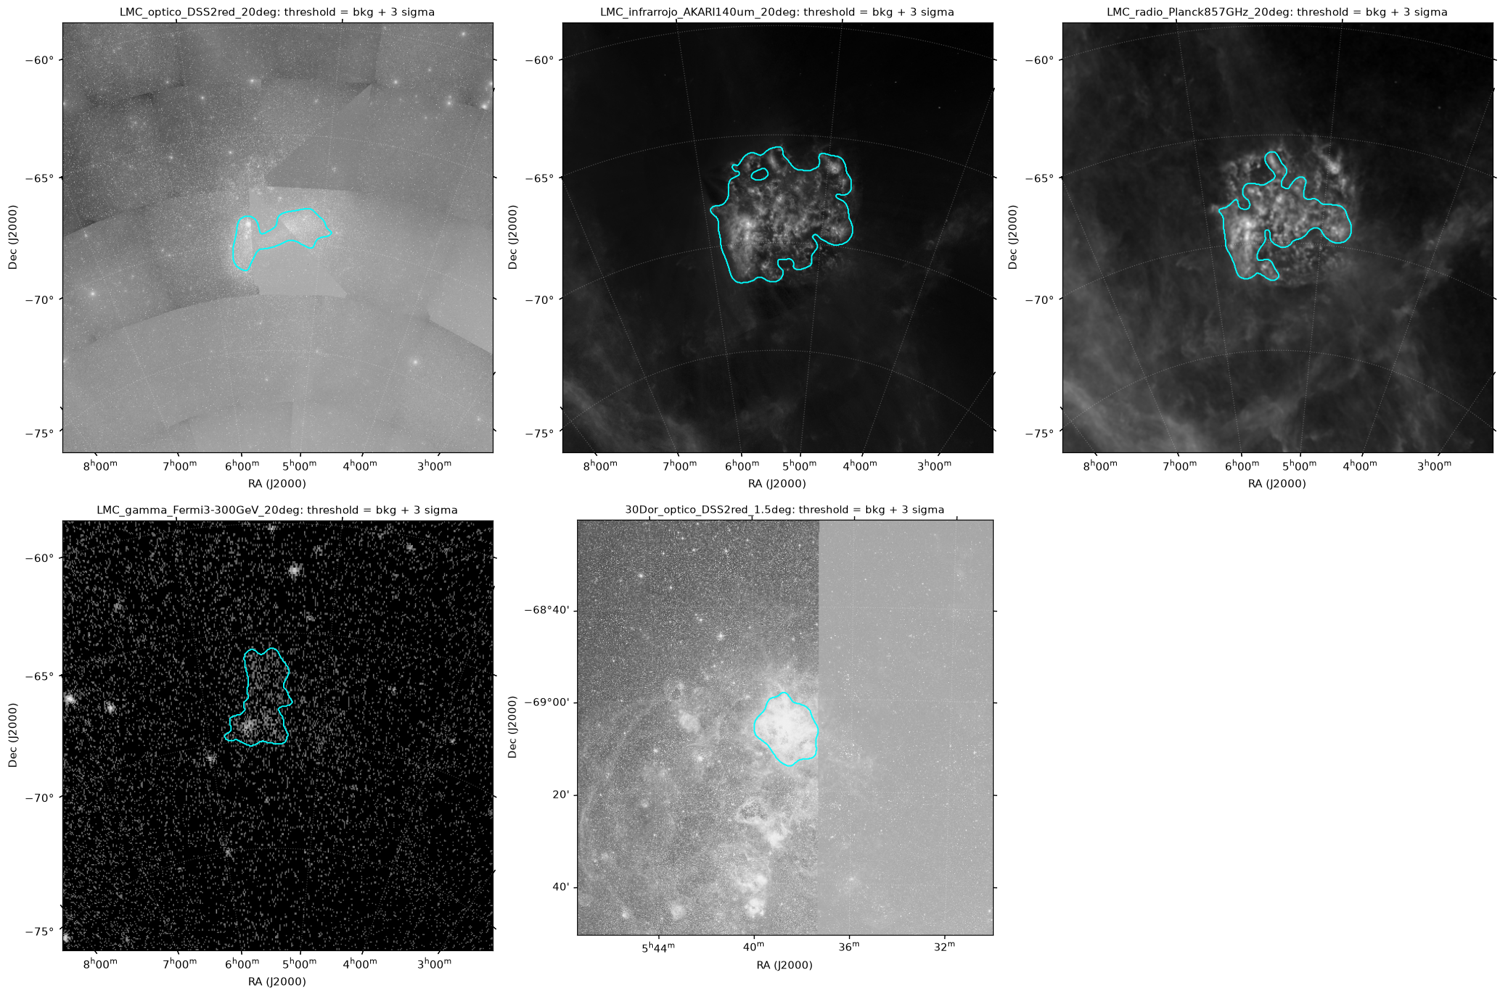
\includegraphics[width=0.58\textwidth]{punto4/panel_medidas_umbral3.png}
\caption{Izquierda: la LMC en óptico; se ven la barra central y el disco difuso. Derecha: contorno de
medida (cian) en óptico, infrarrojo (AKARI \SI{140}{\micro m}), submilimétrico (Planck \SI{857}{GHz}),
radio (Planck \SI{30}{GHz}), rayos gamma (Fermi \SIrange{3}{300}{GeV}) y 30~Doradus.}
\label{fig:bandas}
\end{figure}

\subsection{(a) Diámetro angular en cada imagen}
Se midió de dos formas: con un umbral, tomando la zona más brillante que el fondo $+\,3\sigma$, y
siguiendo el brillo a lo largo de cada eje hasta donde casi se iguala al cielo, como con la herramienta
de distancia de Aladin.
Las medidas se marcaron en Aladin (figura~\ref{fig:reglas}).

\begin{table}[H]
\centering
\caption{Diámetro angular de la LMC en cada banda (eje mayor $\times$ eje menor).}
\label{tab:diam}
\small
\begin{tabular}{lccc}
\toprule
Banda & Umbral ($3\sigma$) & Perfil por los ejes & Referencia \\
\midrule
Óptico & $4.87^\circ \times 2.42^\circ$ & $11.33^\circ \times 8.27^\circ$ & RC3: $10.76^\circ \times 9.16^\circ$ \\
Infrarrojo (AKARI) & $6.98^\circ \times 5.51^\circ$ & $6.43^\circ \times 4.80^\circ$ & -- \\
Submm (Planck 857 GHz) & $6.14^\circ \times 4.54^\circ$ & $6.53^\circ$ (eje mayor) & -- \\
Radio (Planck 30 GHz) & $5.66^\circ \times 5.39^\circ$ & $7.10^\circ \times 5.60^\circ$ & -- \\
Rayos gamma (Fermi) & $5.10^\circ \times 3.08^\circ$\,$^*$ & sin borde definido & -- \\
30 Doradus & $15.5' \times 12.4'$ & $37.5' \times 30.0'$ & SIMBAD: $40' \times 25'$ \\
\bottomrule
\multicolumn{4}{l}{\footnotesize $^*$ Sobre el mapa suavizado ($\sigma = 0.5^\circ$); es una cota superior.}
\end{tabular}
\end{table}

\begin{figure}[H]
\centering
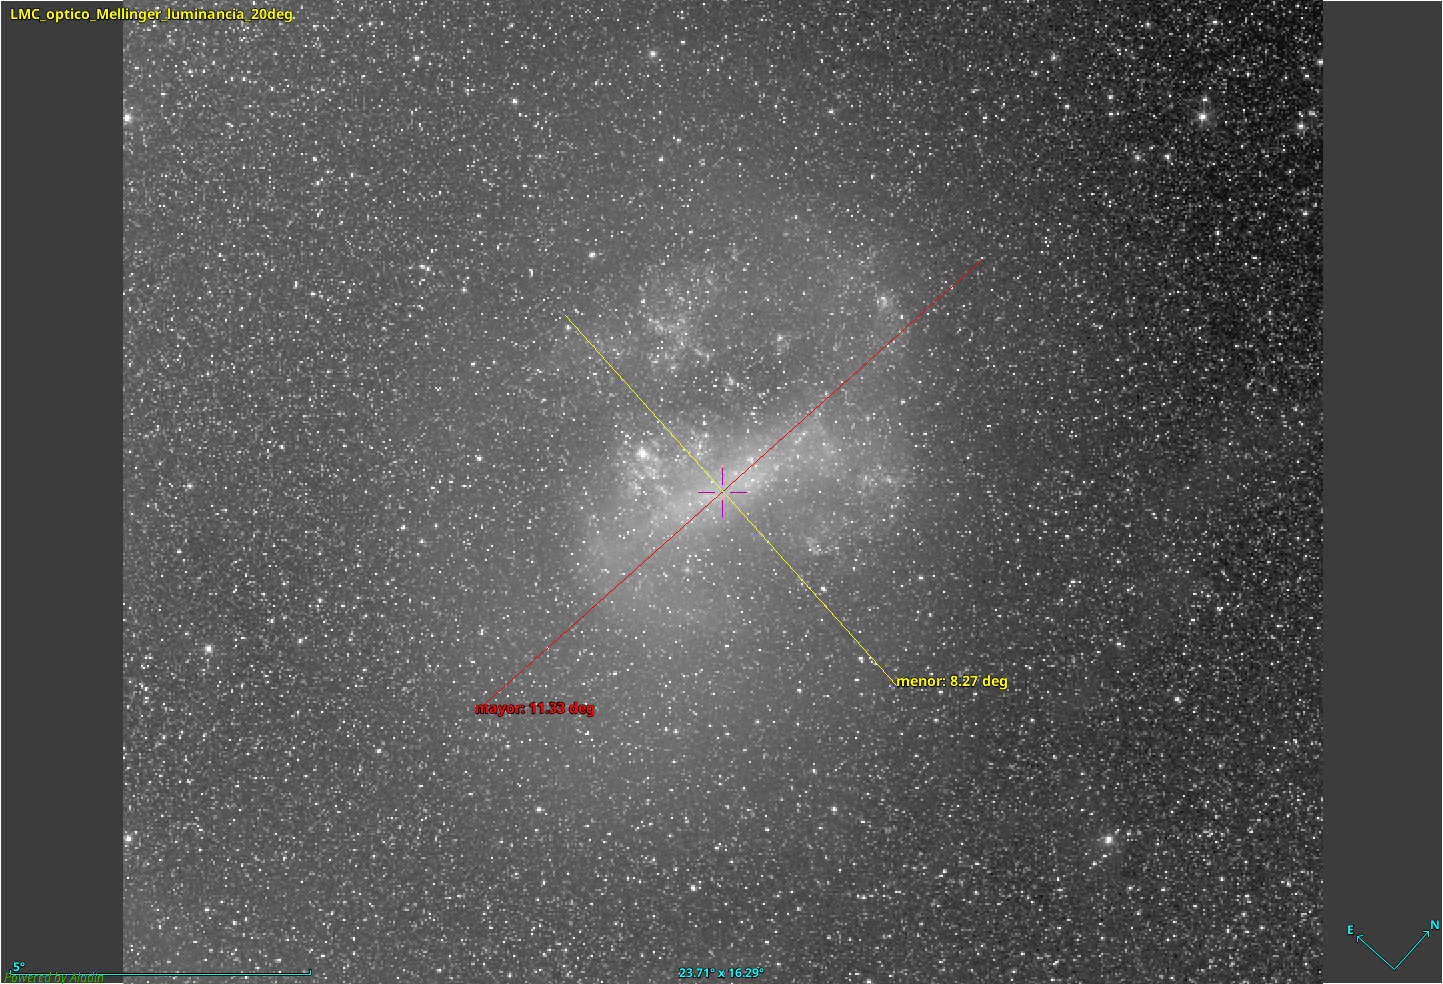
\includegraphics[width=0.32\textwidth]{capturas/aladin_regla_optico.png}
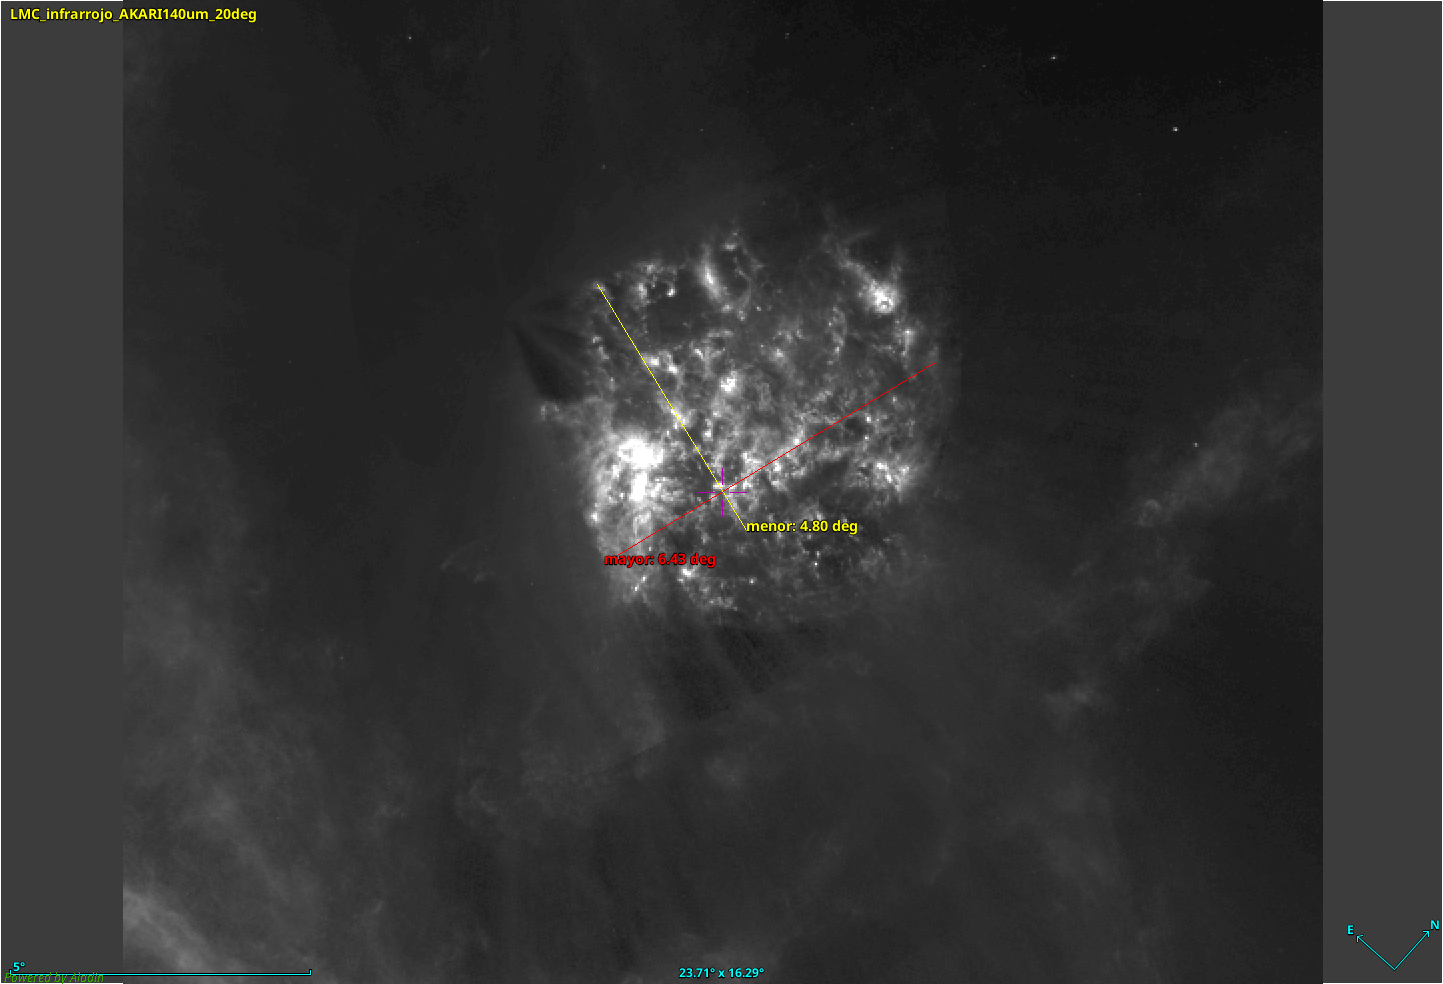
\includegraphics[width=0.32\textwidth]{capturas/aladin_regla_akari.png}
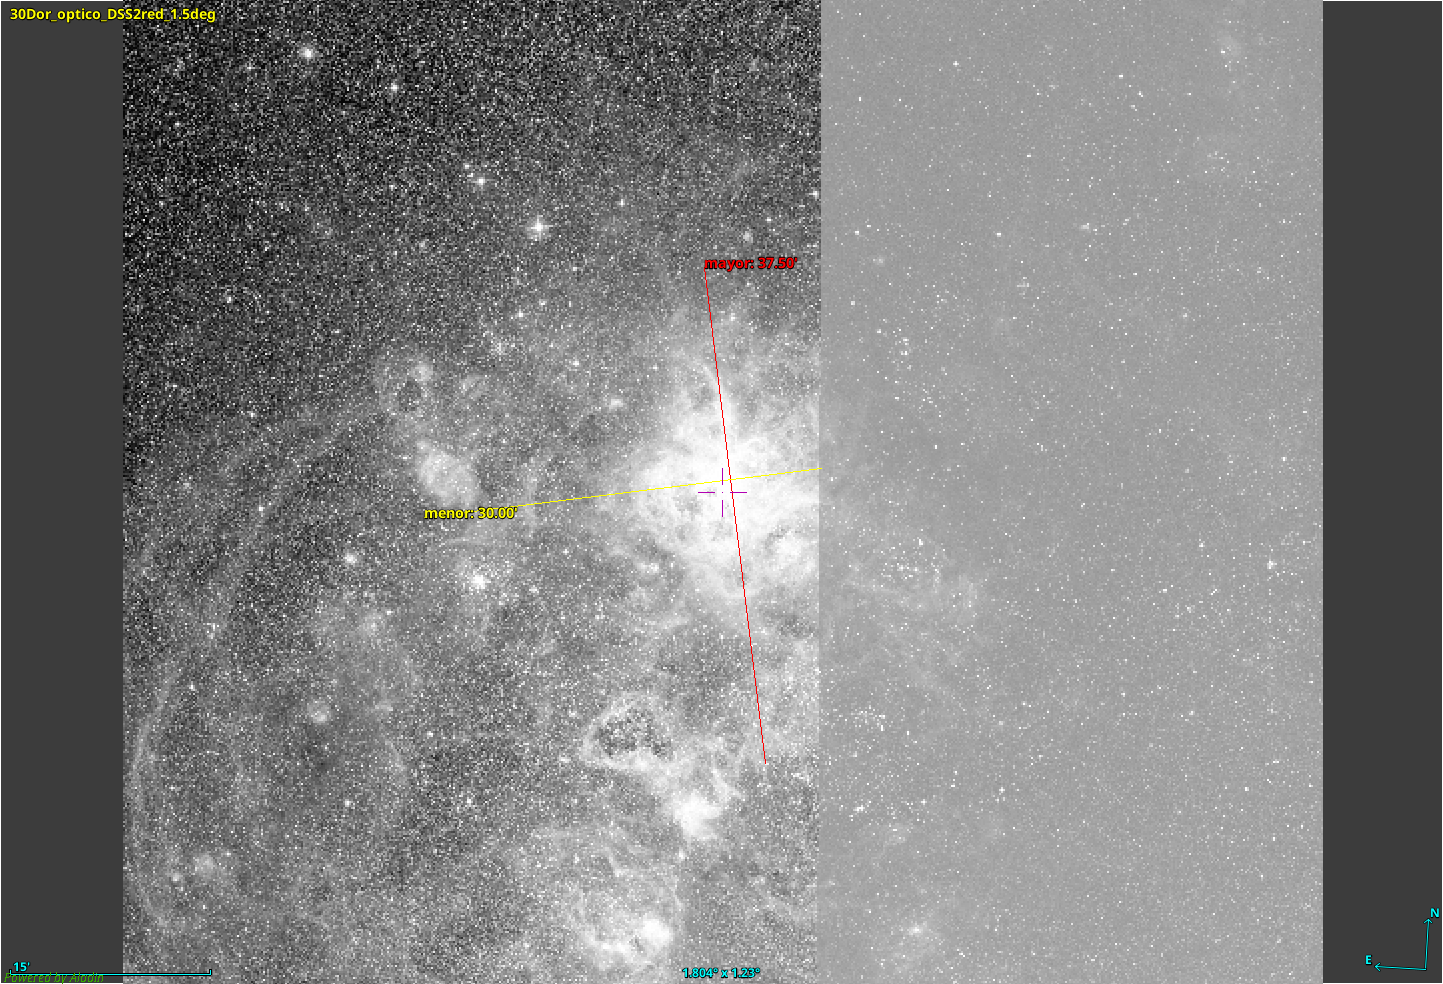
\includegraphics[width=0.32\textwidth]{capturas/aladin_regla_30dor.png}
\caption{Ejes medidos en Aladin (rojo: eje mayor; amarillo: eje menor) en óptico, infrarrojo y
30~Doradus.}
\label{fig:reglas}
\end{figure}

El tamaño cambia según la banda porque cada una ve algo distinto:
\begin{itemize}
  \item en \textbf{óptico}, la luz de las estrellas: la barra brillante y un disco externo débil;
  \item en \textbf{infrarrojo}, el polvo frío calentado por estrellas jóvenes, repartido por todo el disco;
  \item en \textbf{submilimétrico}, polvo aún más frío, mezclado con nubes de polvo de nuestra galaxia;
  \item en \textbf{radio}, el gas ionizado de las regiones de formación estelar, como 30~Doradus;
  \item en \textbf{rayos gamma}, los rayos cósmicos que chocan con el gas. Llegan pocos fotones y la
  emisión solo se distingue al suavizar el mapa.
\end{itemize}
También depende de dónde se ponga el borde. El umbral de $3\sigma$ deja afuera el halo débil:
en óptico mide solo la barra, y en 30~Doradus, solo el núcleo. Con el perfil por los ejes, el tamaño
óptico coincide con el de RC3, y el de 30~Doradus con el de SIMBAD. En infrarrojo y submilimétrico, los
dos criterios coinciden dentro del 8\,\%.

\textbf{Tamaño físico.} Con la aproximación de ángulo pequeño, $D = d\,\theta$ con $\theta$ en radianes
(tabla~\ref{tab:fis}).

\begin{table}[H]
\centering
\caption{Tamaño físico correspondiente, con $d = \SI{50}{kpc}$.}
\label{tab:fis}
\begin{tabular}{lccc}
\toprule
Objeto & $\theta$ & $\theta$ (rad) & $D = \SI{50}{kpc}\cdot\theta$ \\
\midrule
LMC, óptico (eje mayor) & $11.33^\circ$ & 0.1977 & \SI{9.9}{kpc} \\
LMC, infrarrojo, diámetro equivalente (umbral) & $5.98^\circ$ & 0.1044 & \SI{5.2}{kpc} \\
LMC, SIMBAD (eje mayor) & $5.38^\circ$ & 0.0939 & \SI{4.7}{kpc} \\
30 Doradus (eje mayor) & $37.5'$ & 0.01091 & \SI{0.55}{kpc} \\
\bottomrule
\end{tabular}
\end{table}

\subsection{(b) Estrellas masivas de Bonanos et al.\ (2009)}
El catálogo ``IR photometry of massive LMC stars'' \cite{bonanos} (VizieR J/AJ/138/1003 \cite{vizier})
contiene fotometría de 1268 estrellas masivas. No trae una columna B$-$V, así que se calcula como
$\text{Bmag} - \text{Vmag}$. Hay 1135 estrellas con ambas magnitudes. De ellas, 35 tienen colores
físicamente imposibles ($B-V < -0.5$ o $> 2.5$) y se grafican aparte; quedan 1100. Pasamos los datos a
Excel e hicimos el gráfico (figura~\ref{fig:cmd}).

\begin{figure}[H]
\centering
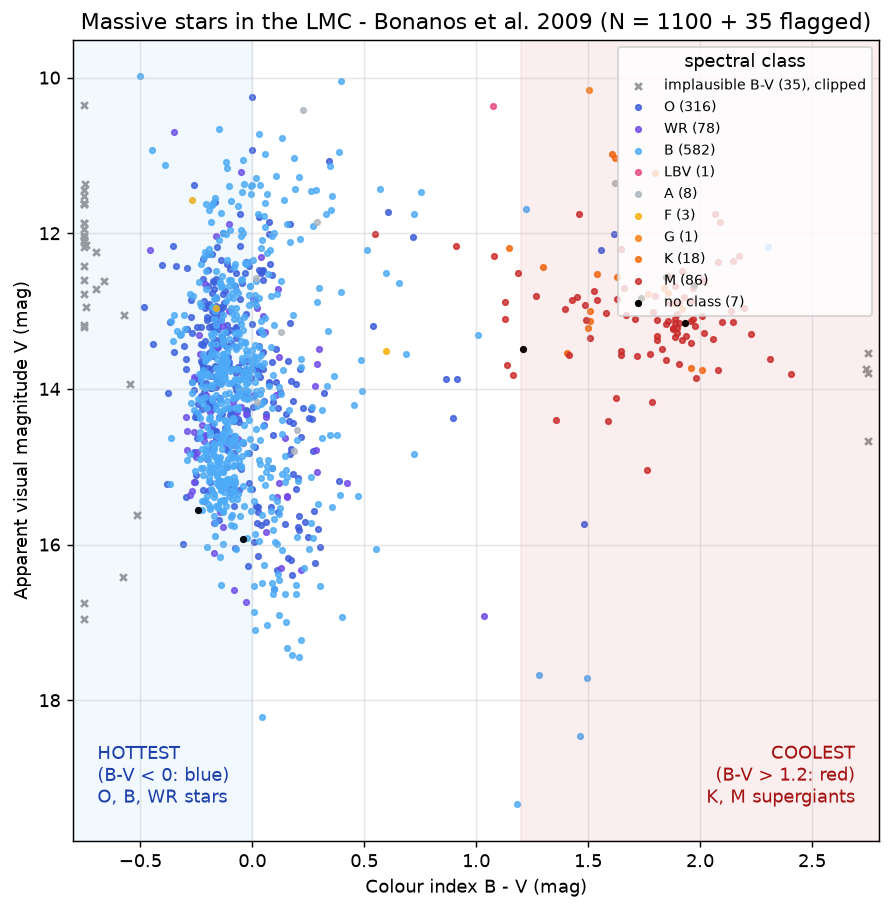
\includegraphics[width=0.49\textwidth]{punto4/Bonanos2009_LMC_V_vs_BV.png}
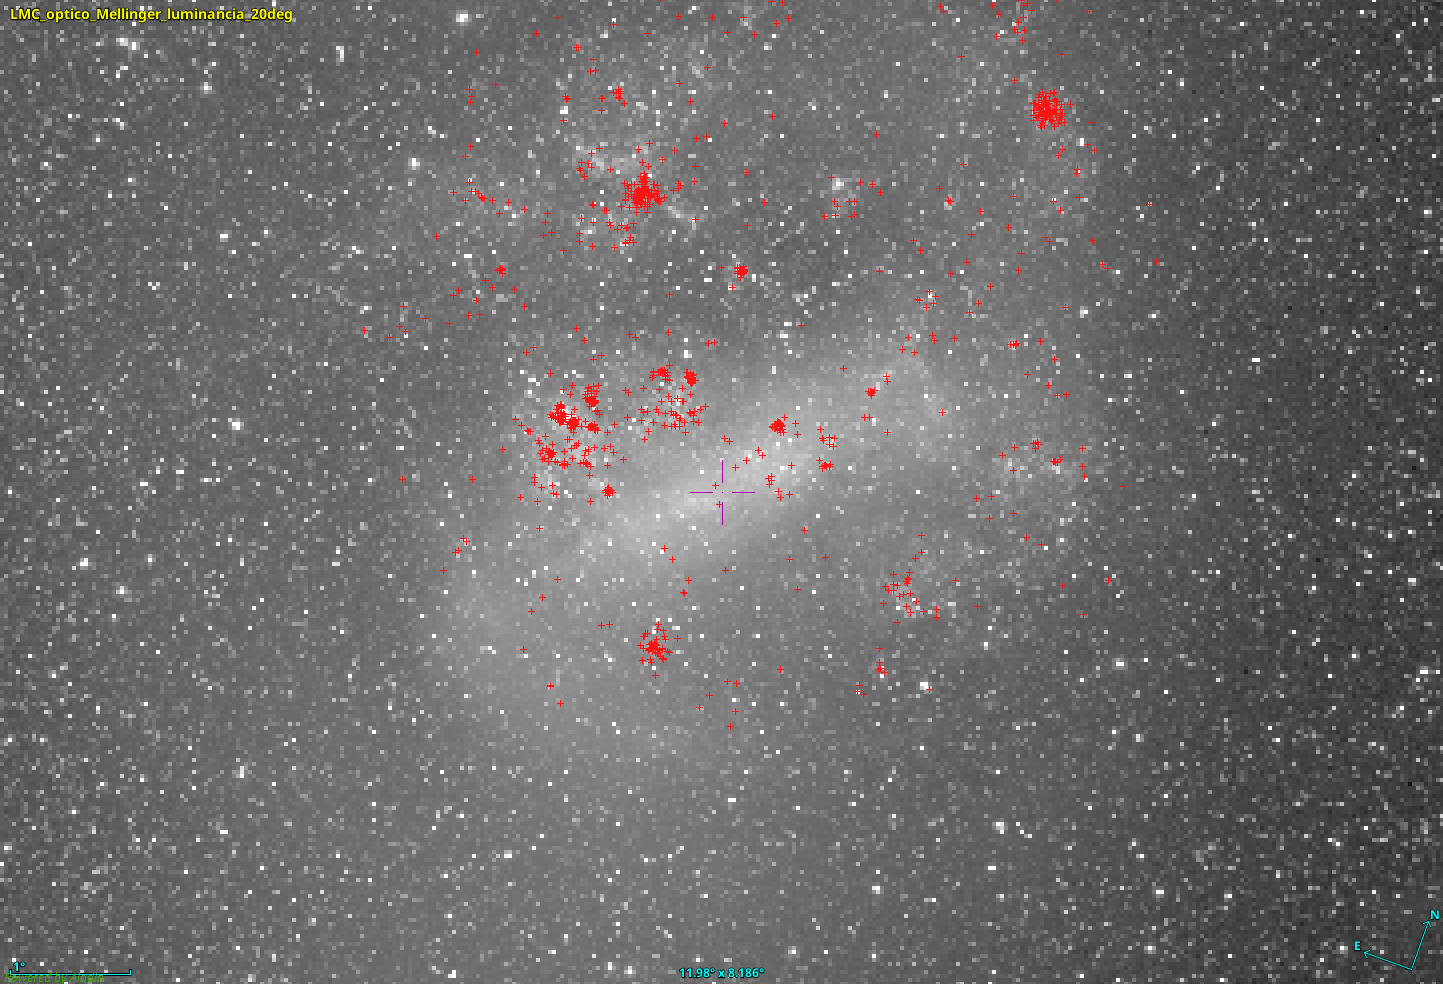
\includegraphics[width=0.49\textwidth]{capturas/aladin_Bonanos2009_sobre_LMC.png}
\caption{Izquierda: magnitud visual aparente V (eje invertido) contra índice de color B$-$V. Derecha:
las estrellas localizadas sobre la imagen en Aladin; se concentran en la barra y en 30~Doradus.}
\label{fig:cmd}
\end{figure}

\subsection{(c) ¿Dónde están las estrellas más frías y las más calientes?}

\begin{table}[H]
\centering
\caption{Índice de color B$-$V por clase espectral.}
\begin{tabular}{lccc}
\toprule
Clase & N & B$-$V medio & Rango \\
\midrule
O & 316 & $-0.05$ & $-0.48$ a $1.62$ \\
Wolf-Rayet & 78 & $-0.06$ & $-0.46$ a $1.03$ \\
B & 582 & $-0.03$ & $-0.50$ a $2.30$ \\
LBV & 1 & $+1.07$ & -- \\
A & 8 & $+0.34$ & $0.02$ a $1.62$ \\
F & 3 & $+0.06$ & $-0.27$ a $0.60$ \\
G & 1 & $+1.50$ & -- \\
K & 18 & $+1.66$ & $1.15$ a $2.01$ \\
M & 86 & $+1.76$ & $0.55$ a $2.41$ \\
Sin clase & 7 & $+1.20$ & $-0.24$ a $1.97$ \\
\midrule
Total & 1100 & & \\
\bottomrule
\end{tabular}
\end{table}

\textbf{a) Las estrellas de superficie más fría están a la derecha} del diagrama, con $B-V$ entre $+1.2$
y $+2.4$. Son supergigantes rojas de tipo K y M, con superficies de unos \SIrange{3500}{4500}{K}. Están
arriba, tan brillantes como las azules, porque son enormes.

\textbf{b) Las más calientes están a la izquierda}, con $B-V \approx 0$ o negativo. Son estrellas O, B y
Wolf-Rayet, con superficies de \SI{20000}{K} a más de \SI{40000}{K}; entre ellas hay supergigantes
azules.

\textbf{¿Por qué?} B mide el brillo en luz azul (\SI{\sim 440}{nm}) y V en luz visual
(\SI{\sim 550}{nm}). Por la ley de Wien, $\lambda_\text{máx} = b/T$ con $b = \SI{2.898e-3}{m.K}$:
\begin{itemize}
  \item una estrella de \SI{30000}{K} tiene su máximo en \SI{97}{nm} (ultravioleta) y brilla más en B
  que en V, así que $B-V < 0$;
  \item una de \SI{3500}{K} tiene su máximo en \SI{828}{nm} y brilla mucho más en V, así que $B-V$ es
  grande.
\end{itemize}
Como todas las estrellas están a la misma distancia (módulo de distancia
$m - M = 5\log_{10}(5000) = 18.5$), el eje V también las ordena por luminosidad.


% =====================================================================
\section{Punto 5: la edad de la Caja de Joyas (NGC 4755)}

\subsection{Datos del cúmulo}
Según SIMBAD \cite{simbad}, NGC~4755 es un cúmulo abierto en $12^\text{h}53^\text{m}39.6^\text{s}$,
$-60^\circ22'16''$ (Cruz del Sur), de $10.3'$ de tamaño, con paralaje $0.462 \pm 0.002$~mas y
distancias publicadas de \SIrange{1.89}{1.99}{kpc}. Sus estrellas más brillantes son supergigantes
azules (tabla~\ref{tab:estrellas}) y una supergigante roja, DU~Cru, que en la foto del taller es la
estrella naranja.

\begin{table}[H]
\centering
\caption{Estrellas más brillantes del cúmulo.}
\label{tab:estrellas}
\begin{tabular}{llcc}
\toprule
Estrella & Tipo espectral & V & B$-$V \\
\midrule
HD 111904 & B9\,Iab (supergigante azul) & 5.77 & 0.28 \\
$\kappa$ Cru & B5\,I (supergigante azul) & 5.94 & 0.18 \\
HD 111990 & B1.5\,I (supergigante azul) & 6.78 & 0.17 \\
BU Cru & B2\,Ib (supergigante azul) & 6.84 & 0.20 \\
DU Cru & M2\,Iab (supergigante roja) & 7.66 & 2.16 \\
CC Cru & B2\,III (gigante azul) & 7.83 & 0.17 \\
\bottomrule
\end{tabular}
\end{table}

\subsection{(1) Centro, límite y estimación de brillo y color}
El centro (X) se ubicó entre las tres concentraciones brillantes del núcleo: la estrella naranja
(DU~Cru), la azul que está justo debajo (BU~Cru) y el grupo azul de abajo a la izquierda
($\kappa$~Cru). El límite se marcó donde la cantidad de estrellas baja al nivel del fondo
(figura~\ref{fig:foto}). Dentro de un cuadrado alrededor del centro se estimó el color de cada
estrella, comparando el tono con la barra O$\ldots$M, y su brillo, comparando el tamaño del punto con
la escala 1--10. Los resultados se volcaron en la hoja de trabajo (figura~\ref{fig:hoja}).

\begin{figure}[H]
\centering
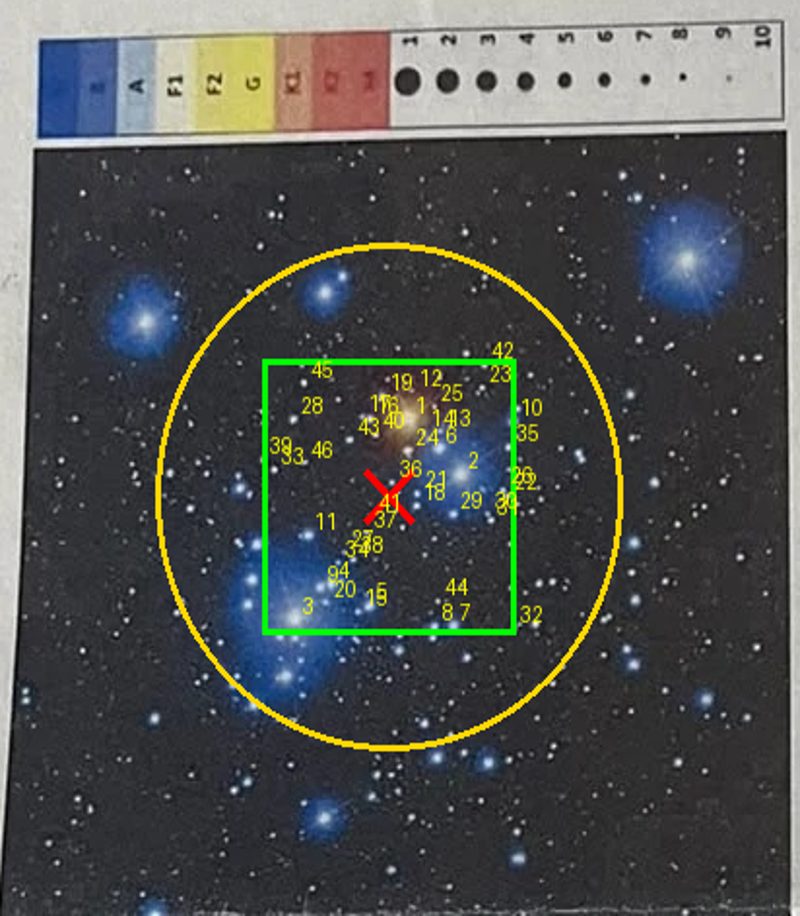
\includegraphics[width=0.48\textwidth]{punto5/pagina2_cumulo_ampliado.png}
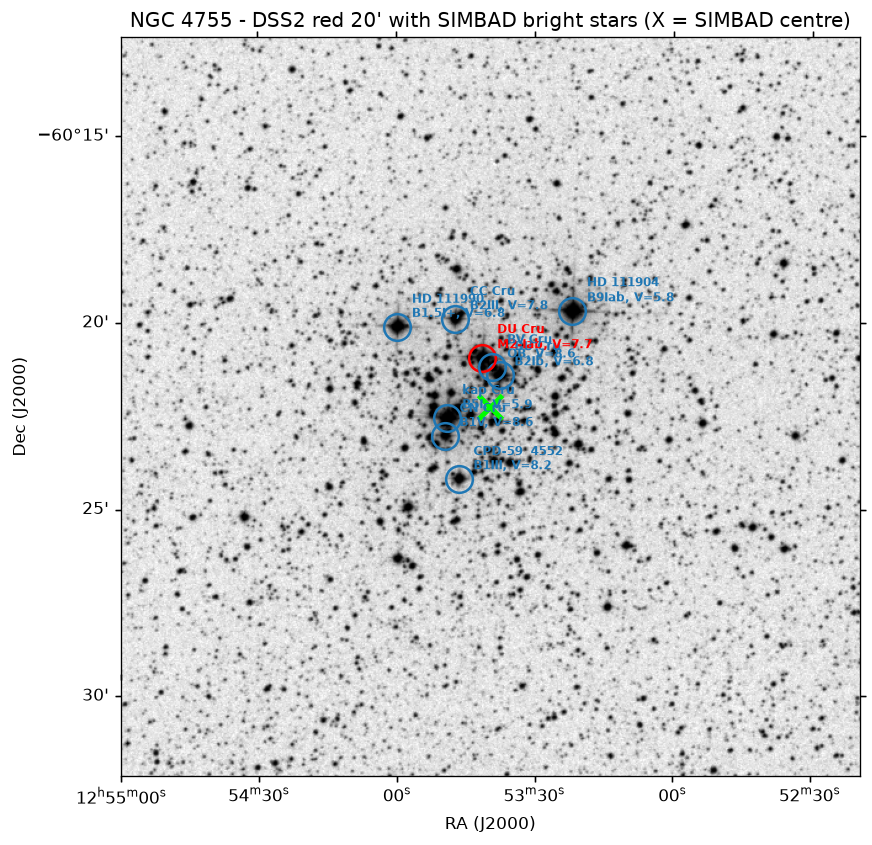
\includegraphics[width=0.48\textwidth]{punto5/NGC4755_DSS2red_estrellas_identificadas.png}
\caption{Izquierda: la imagen del taller con el centro (X), el límite (círculo) y el cuadrado. Derecha:
el mismo cúmulo con sus estrellas brillantes identificadas.}
\label{fig:foto}
\end{figure}

\begin{figure}[H]
\centering
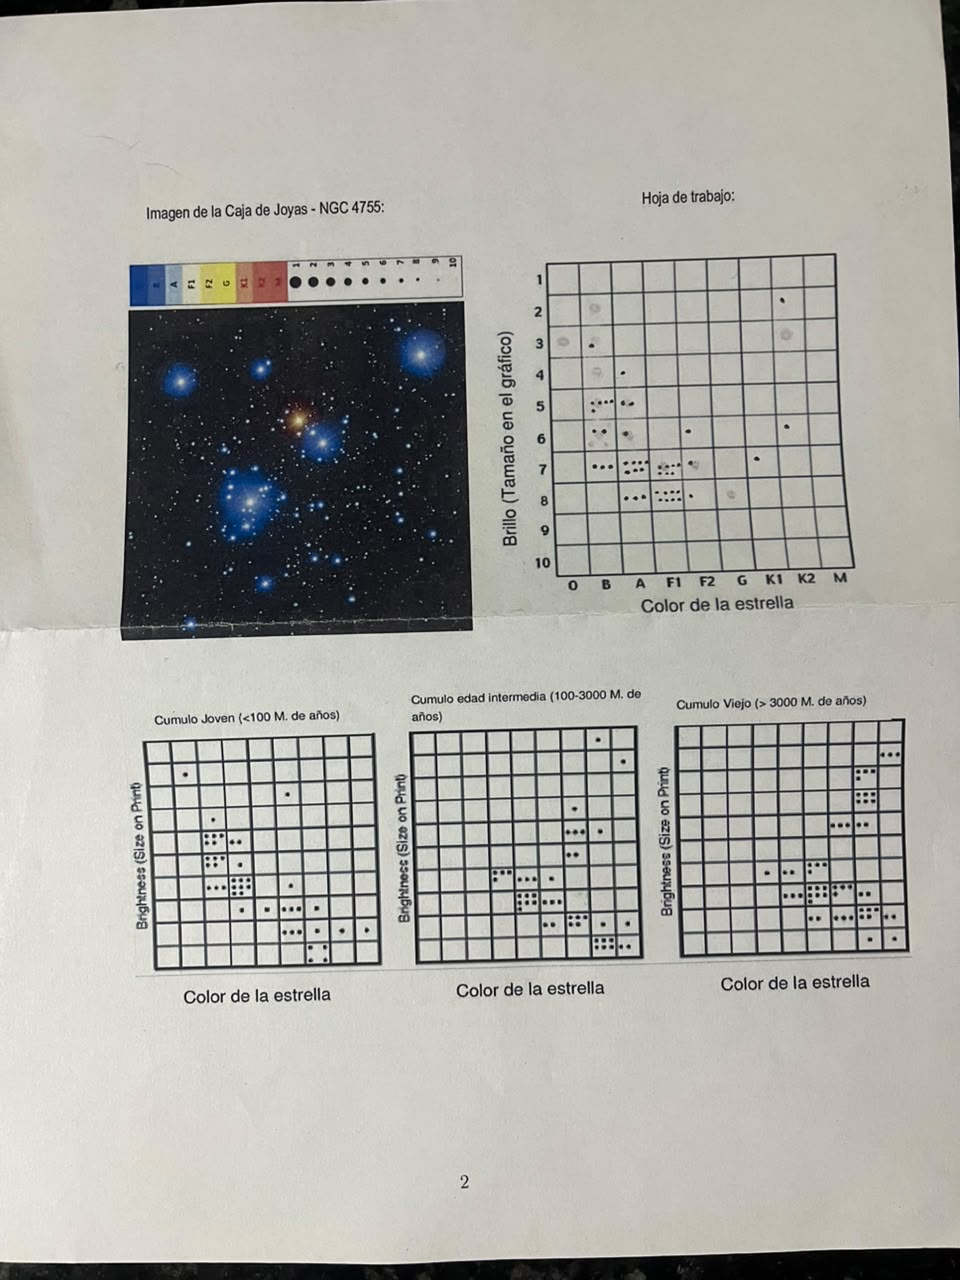
\includegraphics[height=0.62\textheight]{hoja4_punto5.jpg}
\caption{Hoja de trabajo: brillo contra color de las estrellas dentro del cuadrado, junto a los tres
diagramas de referencia.}
\label{fig:hoja}
\end{figure}

\subsection{(2) Estimación de la edad}
Al comparar la hoja de trabajo con los tres diagramas de referencia:
\begin{itemize}
  \item un cúmulo \textbf{joven} ($< 100$ millones de años) tiene estrellas azules muy brillantes
  arriba a la izquierda;
  \item uno de \textbf{edad intermedia} (100 a 3000 millones de años) ya no las tiene y muestra gigantes
  rojas;
  \item uno \textbf{viejo} ($> 3000$ millones de años) solo conserva la parte baja de la secuencia y
  muchas gigantes rojas.
\end{itemize}
La hoja de trabajo de la Caja de Joyas tiene estrellas B muy brillantes arriba a la izquierda, una
secuencia que baja hacia las clases A y F, y una sola supergigante roja. No muestra el grupo de gigantes
rojas de los cúmulos más viejos. Entonces \textbf{la Caja de Joyas es un cúmulo joven, de menos de
100 millones de años}.

Que haya una supergigante roja no cambia esto, porque las estrellas más masivas son las primeras en
volverse gigantes rojas. La literatura da para NGC~4755 una edad de $10 \pm 5$ millones de años
\cite{sanner}, $14 \pm 2$ millones de años \cite{bonatto} y 16 millones de años \cite{piskunov}, lo
que coincide con nuestra estimación.

% =====================================================================
\begin{thebibliography}{99}
\bibitem{simbad} M.~Wenger et al., \emph{The SIMBAD astronomical database}, A\&AS \textbf{143}, 9 (2000).
\bibitem{vizier} F.~Ochsenbein, P.~Bauer y J.~Marcout, \emph{The VizieR database of astronomical
catalogues}, A\&AS \textbf{143}, 23 (2000).
\bibitem{aladin} F.~Bonnarel et al., \emph{The ALADIN interactive sky atlas}, A\&AS \textbf{143}, 33 (2000).
\bibitem{bonanos} A.~Z. Bonanos et al., \emph{Spitzer SAGE infrared photometry of massive stars in the
Large Magellanic Cloud}, AJ \textbf{138}, 1003 (2009).
\bibitem{rc3} G.~de Vaucouleurs et al., \emph{Third Reference Catalogue of Bright Galaxies} (RC3),
Springer, Nueva York (1991).
\bibitem{mellinger} A.~Mellinger, \emph{A color all-sky panorama image of the Milky Way}, PASP
\textbf{121}, 1180 (2009).
\bibitem{akari} Y.~Doi et al., \emph{The AKARI far-infrared all-sky survey maps}, PASJ \textbf{67}, 50
(2015).
\bibitem{planck} Planck Collaboration, \emph{Planck 2018 results. I. Overview and the cosmological
legacy of Planck}, A\&A \textbf{641}, A1 (2020).
\bibitem{fermi} W.~B. Atwood et al., \emph{The Large Area Telescope on the Fermi Gamma-ray Space Telescope
mission}, ApJ \textbf{697}, 1071 (2009).
\bibitem{sanner} J.~Sanner, J.~Brunzendorf, J.-M. Will y M.~Geffert, \emph{Photometric and kinematic
studies of open star clusters. III. NGC 4103, NGC 5281, and NGC 4755}, A\&A \textbf{369}, 511 (2001).
\bibitem{bonatto} C.~Bonatto, E.~Bica, S.~Ortolani y B.~Barbuy, \emph{Detection of Ks-excess stars in
the 14 Myr open cluster NGC 4755}, A\&A \textbf{453}, 121 (2006).
\bibitem{piskunov} A.~E. Piskunov et al., \emph{On the determination of age and mass functions of stars
in young open star clusters from the analysis of their luminosity functions}, MNRAS \textbf{349}, 1449
(2004).
\bibitem{naoj} National Astronomical Observatory of Japan, \emph{Venus at greatest brilliancy} (2017).
\bibitem{earthsky} EarthSky, \emph{Venus at its brightest in the morning sky} (2026).
\end{thebibliography}

\end{document}
